\documentclass[12pt, a4paper]{article}

\usepackage[T2A]{fontenc}
\usepackage[utf8]{inputenc}
\usepackage[russian]{babel}
\usepackage{graphicx}
\usepackage{float}
\usepackage[left=2.5cm, right=2.5cm, top=2cm, bottom=2cm]{geometry}
\usepackage[backend=biber, style=gost-numeric, sorting=none]{biblatex}
\usepackage{hyperref}
\usepackage{amsmath}
\usepackage{amssymb}

\addbibresource{references.bib}

\begin{document}

\begin{titlepage}
    \centering
    \vspace*{\fill}
    \LARGE
    \textbf{Прогнозирование хаотических временных рядов}
    \vspace{2cm}
    \large
    \textbf{Ключевые слова:} временные ряды, система Лоренца,
     прогнозирование, кластеризация, непрогнозируемые точки,
      расширение выборки, метод характерных последовательностей.
    \vspace*{\fill}
\end{titlepage}

\newpage
\section*{Аннотация}
Данная работа посвящена исследованию улучшения точности прогнозирования
 хаотических временных рядов путем расширения обучающей выборки данными
  из схожих динамических систем. В качестве основного метода используется
   алгоритм, основанный на поиске характерных последовательностей (мотивов),
    который эффективен при прогнозировании на несколько шагов вперед, но 
    требователен к объему данных. Исследуется возможность компенсации
     недостатка данных основного ряда за счет добавления временных рядов, 
     сгенерированных системой Лоренца с близкими управляющими параметрами.
      Проведены эксперименты, демонстрирующие, что такой подход позволяет 
      значительно сократить количество непрогнозируемых точек, сохраняя
       при этом приемлемый уровень точности прогноза.
\newpage
\tableofcontents
\newpage

\section{Введение}
Точное предсказание цен акций, погодных условий, потребления
энергии имеет решающее значение для эффективного принятия 
решений на финансовых рынках, при управлении ресурсами,
оптимизациях энергосистем. На данный момент существует
огромное множество способов предсказания временных рядов,
однако большинство из них использует предсказания на один
шаг вперёд. Такой подход показывает свою эффективность
на небольшом количестве шагов предсказания, однако при
предсказании на несколько десятков шагов такие алгоритмы
сталкиваются с «горизонтом прогнозирования» вследствие
экспоненциального возрастания ошибки предсказаний.
Для того чтобы справиться с этой проблемой, был
разработан метод нахождения характерных последовательностей. 
При попытке прогнозирования с помощью этого метода мы сталкиваемся
с отсутствием достаточно большой выборки на реальных данных. Например,
для почти идеального результата на финансовых данных необходимо порядка \(10^9\) наблюдений.

В идеальной ситуации, когда предсказываемое множество имеет 
размерность d и представляет собой d-мерный куб со стороной a, 
для оценки размерности необходимо хотя бы \(N \sim \frac{a^d}{(0.1a)^d} = 10^d\)
точек. В неидеальной ситуации \(N > N_0 \cdot 10^d\), причём константа 
\(N_0 \sim \epsilon_{fr}^{-d}\), где \(\epsilon_{fr}\)---масштаб фрактальности,
может быть довольно значительной. Например, в аттракторе Хенона \(\epsilon_{fr} \sim 0.1\). 
Но, даже в случае, если существует достаточно большой временной ряд, возникает 
проблема стационарности данных, т. е. динамическая система может изменять свои свойства с течением времени.
\section*{Ключевые идеи метода}

Алгоритм строит \textit{множество возможных предсказаний} $\hat{S}_{t+h} = \{\hat{y}_{t+h}^{(1)}, \dots, \hat{y}_{t+h}^{(N_{t+h})}\}$ для каждой предсказываемой точки. Это достигается за счёт:
\begin{enumerate}
    \item использования \textit{обобщённых $z$-векторов} (векторов несмежных наблюдений);
    \item \textbf{объединения $z$-векторов, сгенерированных из нескольких схожих временных рядов (основного и вспомогательных)};
    \item кластеризации объединённых выборок по шаблонам для получения \textit{мотивов};
    \item объединения предсказаний, полученных по множеству шаблонов;
    \item введения понятия \textit{непредсказуемых точек}.
\end{enumerate}

\section*{Генерация обучающих выборок по шаблонам из нескольких рядов}

Пусть дано множество временных рядов $\mathcal{Y} = \{Y^{(0)}, Y^{(1)}, \dots, Y^{(M)}\}$, где $Y^{(0)}$ — основной (целевой) ряд, а $Y^{(1)}, \dots, Y^{(M)}$ — вспомогательные ряды, сгенерированные динамическими системами с близкими параметрами.

Шаблон — это вектор расстояний между индексами наблюдений:
\[
\boldsymbol{k} = (k_1, k_2, \dots, k_{L-1}), \quad 1 \leq k_j \leq K_{\max},
\]
где $L$ — длина $z$-вектора, $K_{\max}$ — максимальный шаг между соседними наблюдениями в шаблоне.

Для каждого ряда $Y^{(m)} = \{y^{(m)}_0, y^{(m)}_1, \dots\} \in \mathcal{Y}$ и для каждого шаблона $\boldsymbol{k}$ генерируется своя выборка обобщённых $z$-векторов:
\[
\mathbf{z}_{t}^{(m, \boldsymbol{k})} = \bigl(y^{(m)}_t,\ y^{(m)}_{t+k_1},\ y^{(m)}_{t+k_1+k_2},\ \dots,\ y^{(m)}_{t + k_1 + \dots + k_{L-1}}\bigr).
\]

Ключевым шагом является \textbf{объединение} всех выборок, соответствующих одному и тому же шаблону $\boldsymbol{k}$, но полученных из разных рядов:
\[
\mathcal{Z}^{(\boldsymbol{k})} = \bigcup_{m=0}^{M} \left\{ \mathbf{z}_{t}^{(m, \boldsymbol{k})} \right\}.
\]
Таким образом, для каждого шаблона $\boldsymbol{k} \in \aleph(L, K_{\max})$ формируется одна, но значительно расширенная обучающая выборка $\mathcal{Z}^{(\boldsymbol{k})}$.

\section*{Кластеризация и формирование мотивов}

Каждая объединённая выборка $\mathcal{Z}^{(\boldsymbol{k})}$, соответствующая шаблону $\boldsymbol{k}$, кластеризуется отдельно с использованием модифицированного алгоритма Уишарта. Центры полученных кластеров интерпретируются как \textit{мотивы}, которые теперь кодируют типичную динамику не одного, а целого семейства схожих систем.

Множество мотивов для шаблона $\alpha = (k_{\alpha 1}, \dots, k_{\alpha L-1})$ обозначается как:
\[
\Psi_\alpha = \{C_\alpha\}, \quad C_\alpha = (\eta_{\alpha 1}, \eta_{\alpha 2}, \dots, \eta_{\alpha L}).
\]
Полное множество мотивов для всех шаблонов: $\Psi = \{(\alpha, \Psi_\alpha)\},\ \alpha \in \aleph(L, K_{\max})$.

Этот подход позволяет эффективно компенсировать недостаток данных в основном ряде за счёт статистически схожих паттернов из вспомогательных рядов, при условии, что все системы генерируют топологически эквивалентные аттракторы.
\subsection{Изучение системы Лоренца}

В качестве исследуемого ряда был выбран ряд Лоренца, который обладает фрактальной размерностью около 2. Основной ряд \(Y\) получен при стандартных параметрах: \(r = 28\), \(\sigma = 10\), \(b = 8/3\). Поведение системы Лоренца существенно зависит от значения параметра \(r\). Были обнаружены следующие характерные режимы:
\begin{enumerate}
    \item При \(r < 1\): система имеет единственную стационарную точку (0,0,0).
    \item При \(1 < r < 13.926\): появляются три стационарные точки.
    \item При \(r \approx 13.926\): возникают гомоклинические орбиты.
    \item При \(13.926 < r < 24.06\): наблюдается метастабильный хаос, хаотическое множество растёт, оставаясь неустойчивым и непритягивающим.
    \item При \(24.06 < r < 24.74\): аттрактор становится притягивающим, сохраняя две устойчивые точки.
    \item При \(r > 24.74\): формируется единственный глобальный странный аттрактор.
    \item При \(r > 50\): появляются устойчивые орбиты.
    \item При \(144 < r < 167\): система демонстрирует две периодические орбиты.
    \item При \(r > 167\): возникает прерывистый хаос с чередованием хаотических и периодических режимов.
\end{enumerate}\section{Визуальный анализ и характеристика данных}

При работе с хаотическими системами необходимо четко разделять два типа различий, возникающих при изменении управляющих параметров.

\begin{enumerate}
    \item \textbf{Качественные изменения}, происходящие в точках бифуркации. В этих точках происходит фундаментальная перестройка динамики системы, и форма (топология) аттрактора кардинально меняется, например, хаотический аттрактор может смениться устойчивой периодической орбитой.
    \item \textbf{Количественные изменения}, наблюдаемые между точками бифуркаций. В этом случае аттрактор сохраняет свою топологическую структуру, однако меняются его метрические свойства. Ключевым изменением является скорость экспоненциального расхождения изначально близких траекторий: как правило, чем больше разница в параметрах (\(\Delta r\)), тем быстрее расходятся траектории.
\end{enumerate}

На Рис. \ref{fig:lorenz_comparison} представлены участки траекторий, иллюстрирующие именно количественные различия. Поскольку все выбранные для эксперимента значения параметра \(r\) находятся в зоне устойчивого хаоса, форма аттрактора остается неизменной.

\begin{figure}[htbp]
    \centering
    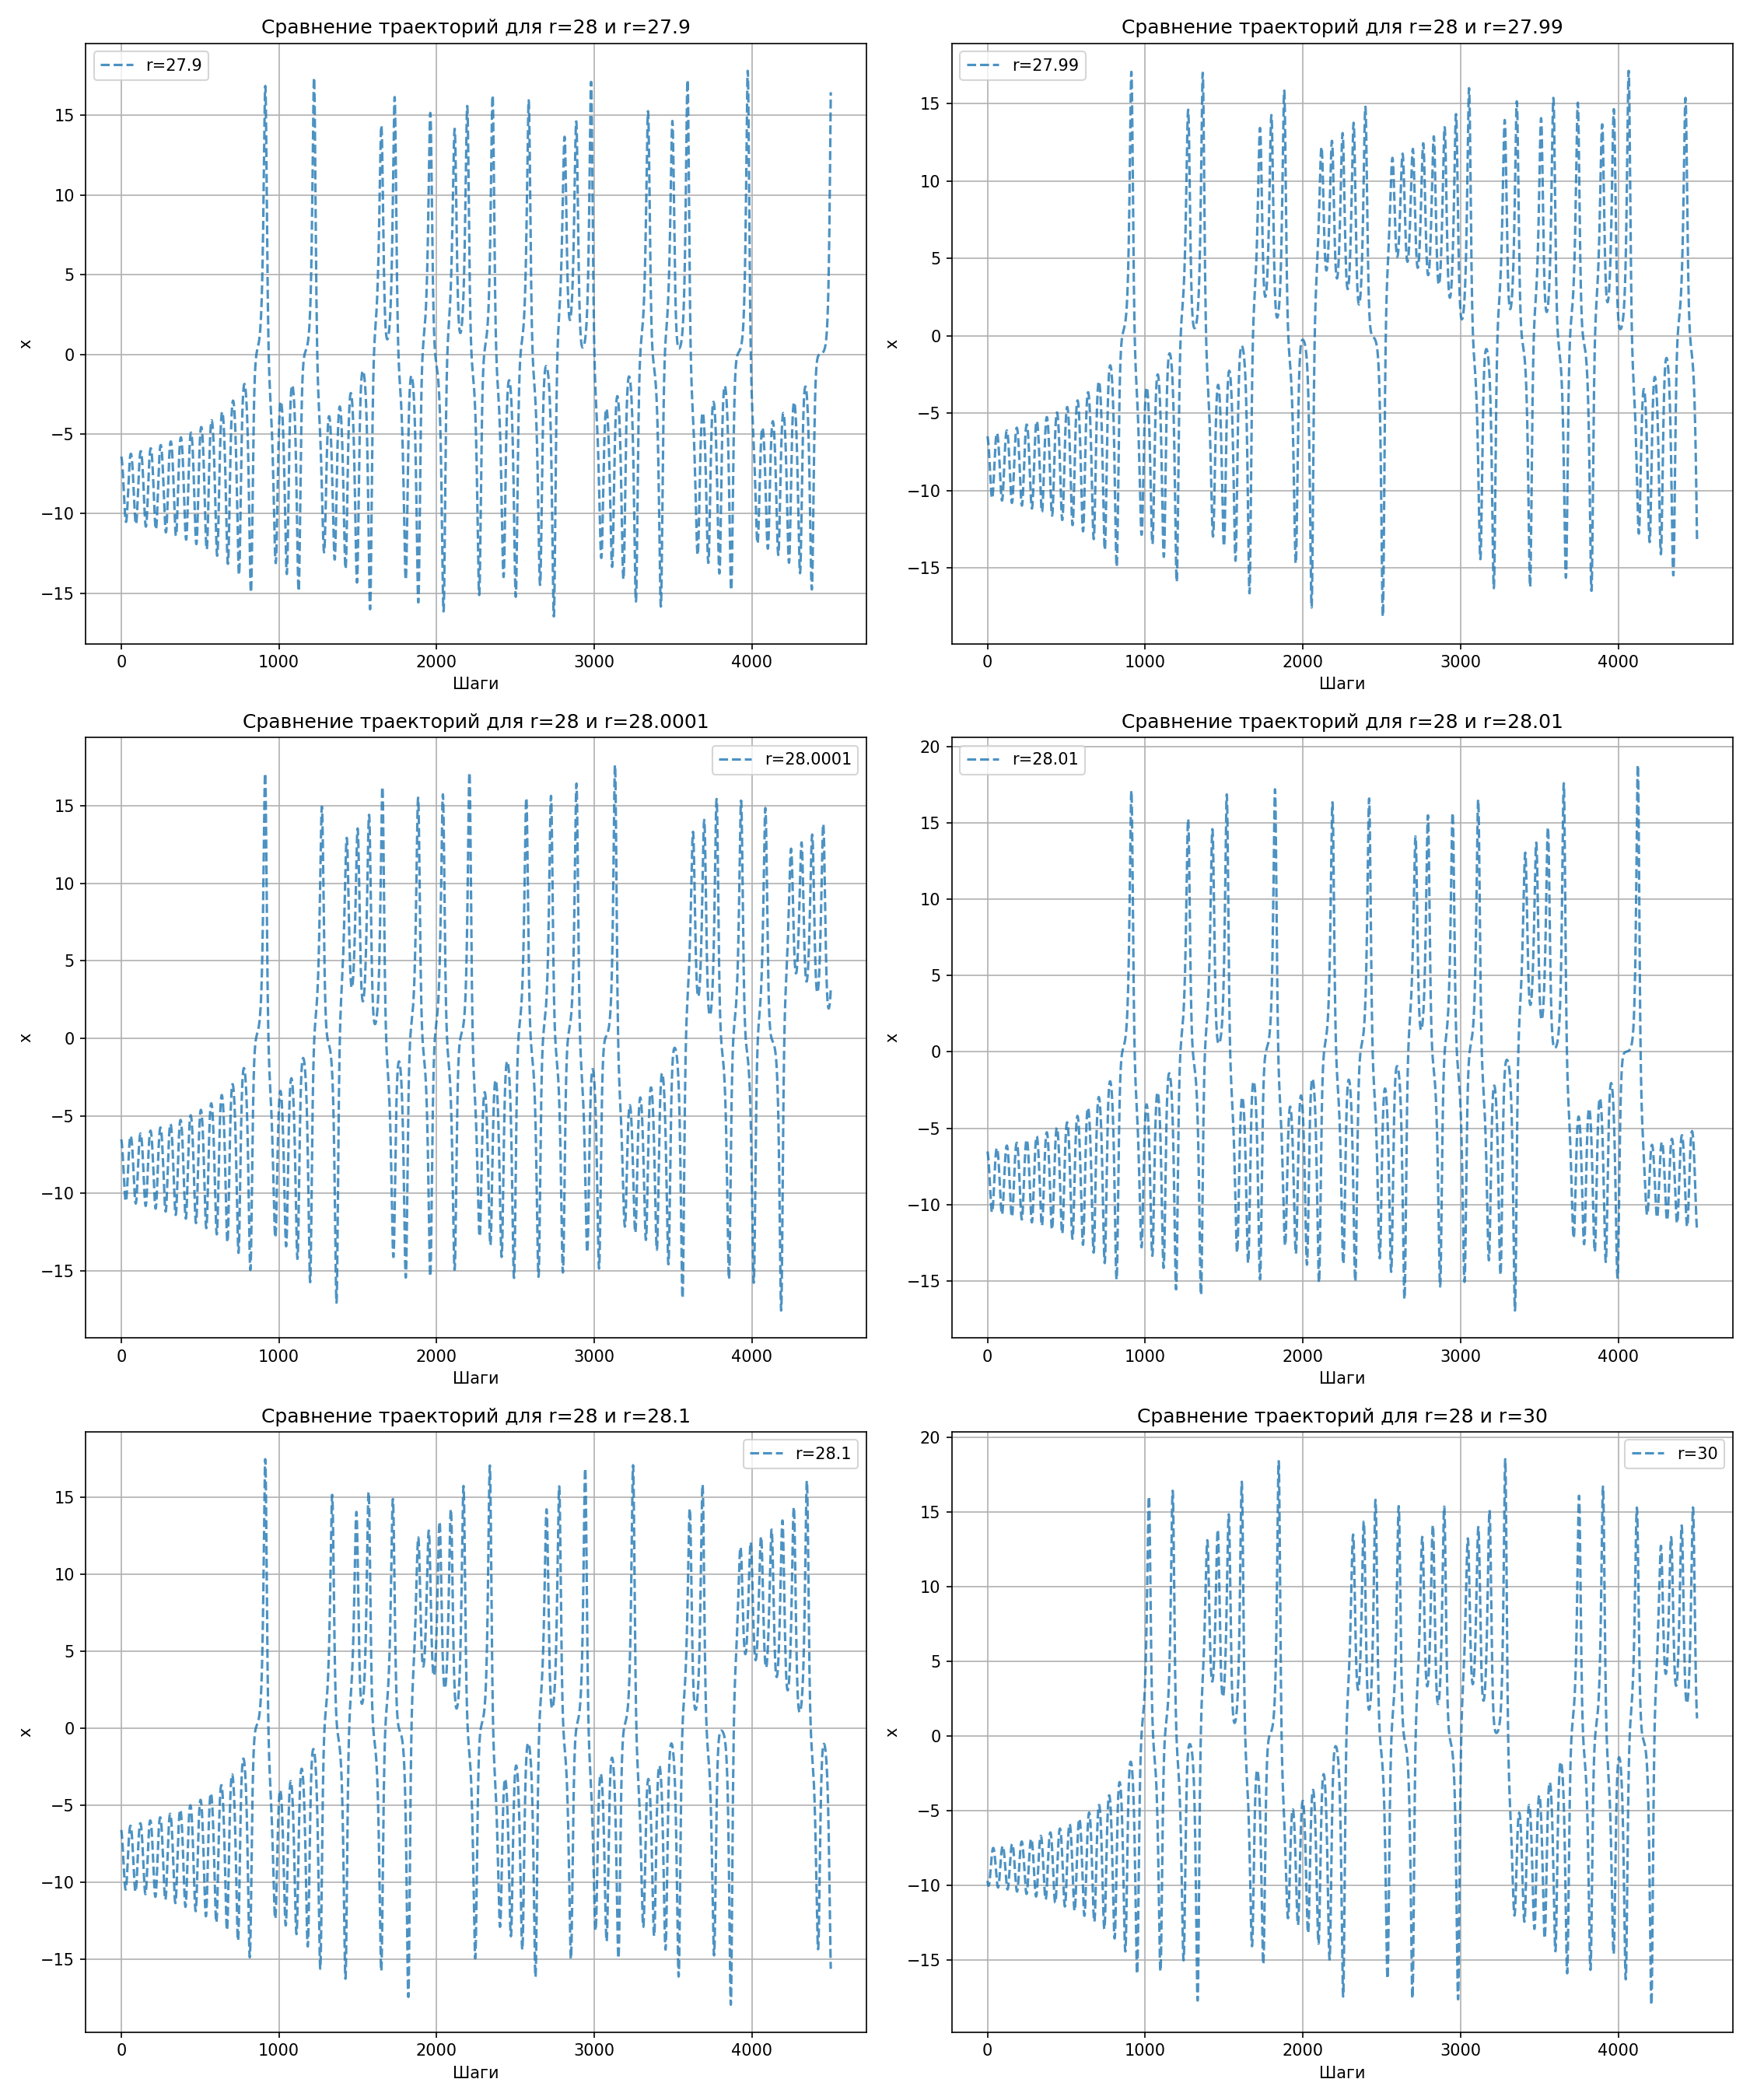
\includegraphics[width=\textwidth]{../dtw/rows.png} 
    \caption{Сравнение участков траекторий системы Лоренца. Все представленные ряды находятся в области одного и того же странного аттрактора, поэтому его топологическая форма сохраняется. Однако визуально заметно, что при большем отклонении параметра \(r\) от базового значения \(r=28\), расхождение траекторий становится более быстрым и выраженным.}
    \label{fig:lorenz_comparison}
\end{figure}

Основополагающая гипотеза данного исследования заключается в том, что метод прогнозирования, 
основанный на поиске локальных паттернов (мотивов), эффективен до тех пор, пока базовый и
 вспомогательный ряды генерируются системами с топологически эквивалентными аттракторами. 
 В этом случае мотивы обеих систем статистически схожи, что позволяет использовать
  мотивы из вспомогательного ряда для прогнозирования основного.

Тем не менее, количественные различия, в частности увеличенная скорость расхождения траекторий 
при большом \(\Delta r\), могут снижать точность прогноза. Даже если идентичный мотив найден,
 последующее развитие траектории в двух системах будет отличаться сильнее, что может приводить
  к увеличению ошибки. В следующих разделах данная зависимость между величиной \(\Delta r\) 
  и метриками качества прогноза будет исследована численно.
\section{Обзор литературы}

Основой для настоящего исследования служат работы В.А. Громова и Ф.С. Баранова [6]
, в которых предложен метод прогнозирования хаотических временных рядов,
 основанный на поиске характерных последовательностей (мотивов).
  Суть подхода заключается в реконструкции фазового пространства
   системы по наблюдаемому временному ряду и последующей кластеризации 
   векторов состояний для выявления повторяющихся паттернов динамики.

Ключевой особенностью метода является использование множества мотивов, 
что порождает набор возможных прогнозных значений для каждой точки.
 Для получения единого прогноза (унификации) в предыдущих работах
  рассматривались различные подходы, включая вычисление среднего
   значения, применение взвешенного усреднения (в зависимости от длины прогноза или расстояния
    до центра кластера) и выбор центра наиболее крупного кластера из возможных прогнозов.

Важнейшим аспектом, отличающим данный подход, является концепция 
непрогнозируемых точек. Она позволяет алгоритму оценивать собственную уверенность
 и воздерживаться от прогноза в ситуациях высокой неопределенности, 
 что повышает надежность модели. Для идентификации таких точек применялись 
 как статистические критерии (энтропия множества прогнозных значений, его 
 мультимодальность, ширина интерквантильного размаха), так и более сложные 
 классификаторы на основе методов машинного обучения, включая логистическую регрессию,
  метод опорных векторов (SVM), деревья решений, k-NN, многослойные перцептроны (MLP) и их ансамбли.

Исследования показали высокую эффективность метода: алгоритм демонстрировал 
практически постоянную ошибку прогноза (MAE, RMSE) даже при увеличении 
горизонта до 100 шагов вперед, что достигалось за счет экспоненциального
 роста числа точек, классифицируемых как непрогнозируемые. Особое значение
  для настоящей работы имеет исследование [5], в котором изучалось влияние 
  
  размера обучающей выборки на точность. Было установлено, что при увеличении о
  бъема данных из *исходного* ряда ошибка прогноза убывала логарифмически. Однако 
  вопрос о том, можно ли компенсировать недостаток данных за счет добавления 
  выборок из *других, но схожих по динамике* систем, оставался открытым.
 Данная работа направлена на исследование именно этой возможности.
 \section{Основная часть: Эксперименты и результаты}
\subsection{Эксперимент 1: Влияние размера и состава обучающей выборки}
\subsubsection{Описание эксперимента}
Основной целью исследования являлась количественная оценка влияния расширения обучающей выборки на точность прогнозирования. В качестве базового временного ряда использовалась система Лоренца ($\sigma$ = 10, r = 28, b = 8/3). К исходной выборке из 10 000 точек базового ряда итеративно добавлялись данные из вспомогательного ряда, сгенерированного с параметром `r`, незначительно отличающимся от базового, до достижения общего размера выборки в 30 000 точек. На каждом шаге для смешанной выборки выполнялось прогнозирование на 10 шагов вперед и оценивались метрики: RMSE, MAPE и доля непрогнозируемых точек (NP). Для оценки эффективности метрики RMSE и MAPE были нормализованы относительно результатов, полученных на гомогенной выборке (состоящей только из данных базового ряда) аналогичного размера.

\subsubsection{Анализ результатов}
\begin{figure}[htbp]
    \centering
    
\includegraphics[width=\textwidth]{../Size_experiment/metrics_vs_general_size_best_experiments.png}
    \caption{Основное исследование: Зависимость метрик от размера выборки для 
    случаев эффективного расширения (deviation = 0.1, 0.0001, -0.1, -0.1).}
    \label{fig:main_exp}
\end{figure}

\paragraph{Анализ случаев улучшения метрик (Рис. \ref{fig:main_exp}):} Для вспомогательных рядов с параметрами `r`, близкими к 28, наблюдается значительное (до 6 раз) снижение доли непрогнозируемых точек, а также снижение RMSE в два раза. При этом метрики точности RMSE и MAPE остаются на уровне, сопоставимом с базовым случаем, или улучшаются. Это подтверждает гипотезу о том, что добавление данных из близких динамических систем повышает робастность модели без существенной потери точности.

\begin{figure}[htbp]
    \centering
    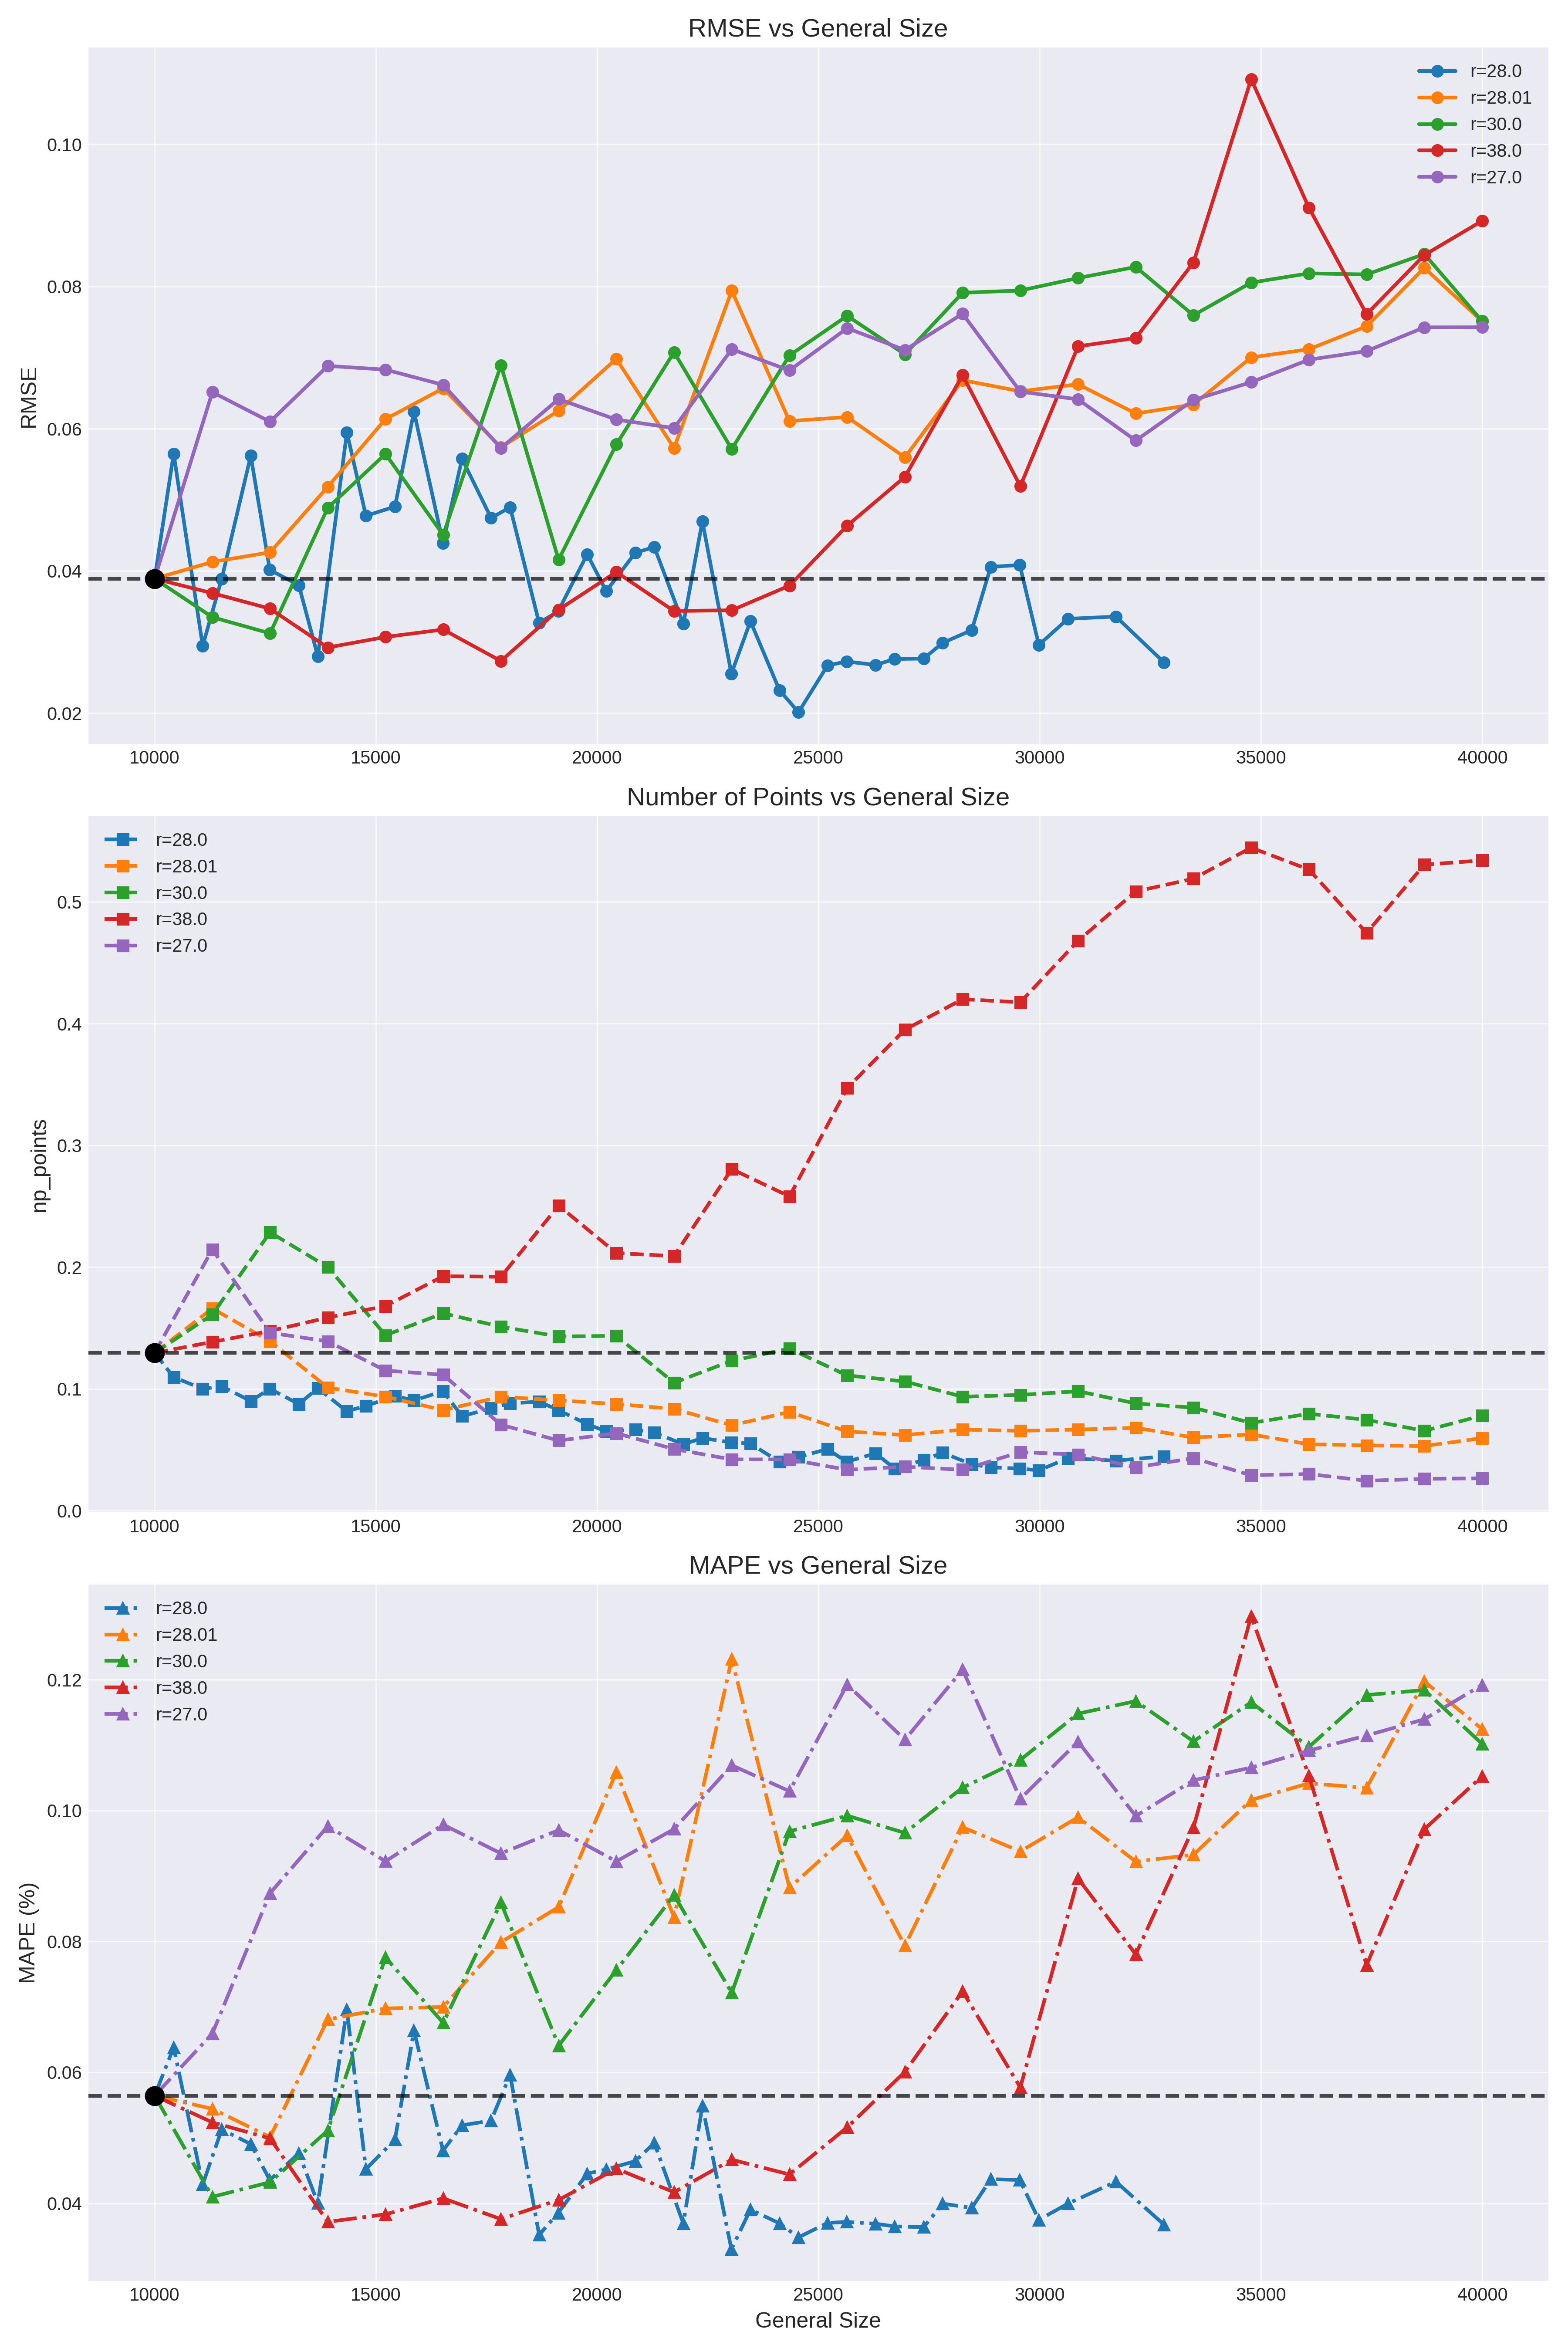
\includegraphics[width=\textwidth]{../Size_experiment/unlucky_experiments.png}
    \caption{Исследование случаев неэффективного расширения (deviation = 0.01, 2, 10, -1).}
    \label{fig:unlucky_exp}
\end{figure}

\paragraph{Анализ случаев ухудшения метрик (Рис. \ref{fig:unlucky_exp}):}
 Когда параметр `r` вспомогательного ряда значительно отличался от базового,
  снижение количества непрогнозируемых точек происходило ценой резкого роста
   ошибок RMSE и MAPE. Это указывает на деградацию качества прогноза при 
   смешивании данных из систем с существенно различной динамикой. Кроме
    того, не все случаи с близкими параметрами приводят к улучшению: 
    например, при добавлении данных с r=28.01 предсказание не улучшается
     и остается на уровне базовой выборки из 5000 точек, без снижения NP или RMSE.

\subsection{Эксперимент 2: Прогноз без использования основного ряда}
\subsubsection{Описание эксперимента}
Данный эксперимент проверял гипотезу о возможности прогнозирования 
целевого ряда с использованием обучающей выборки, состоящей исключительно из данных вспомогательных рядов.

\subsubsection{Анализ результатов}
\begin{figure}[htbp]
    \centering
    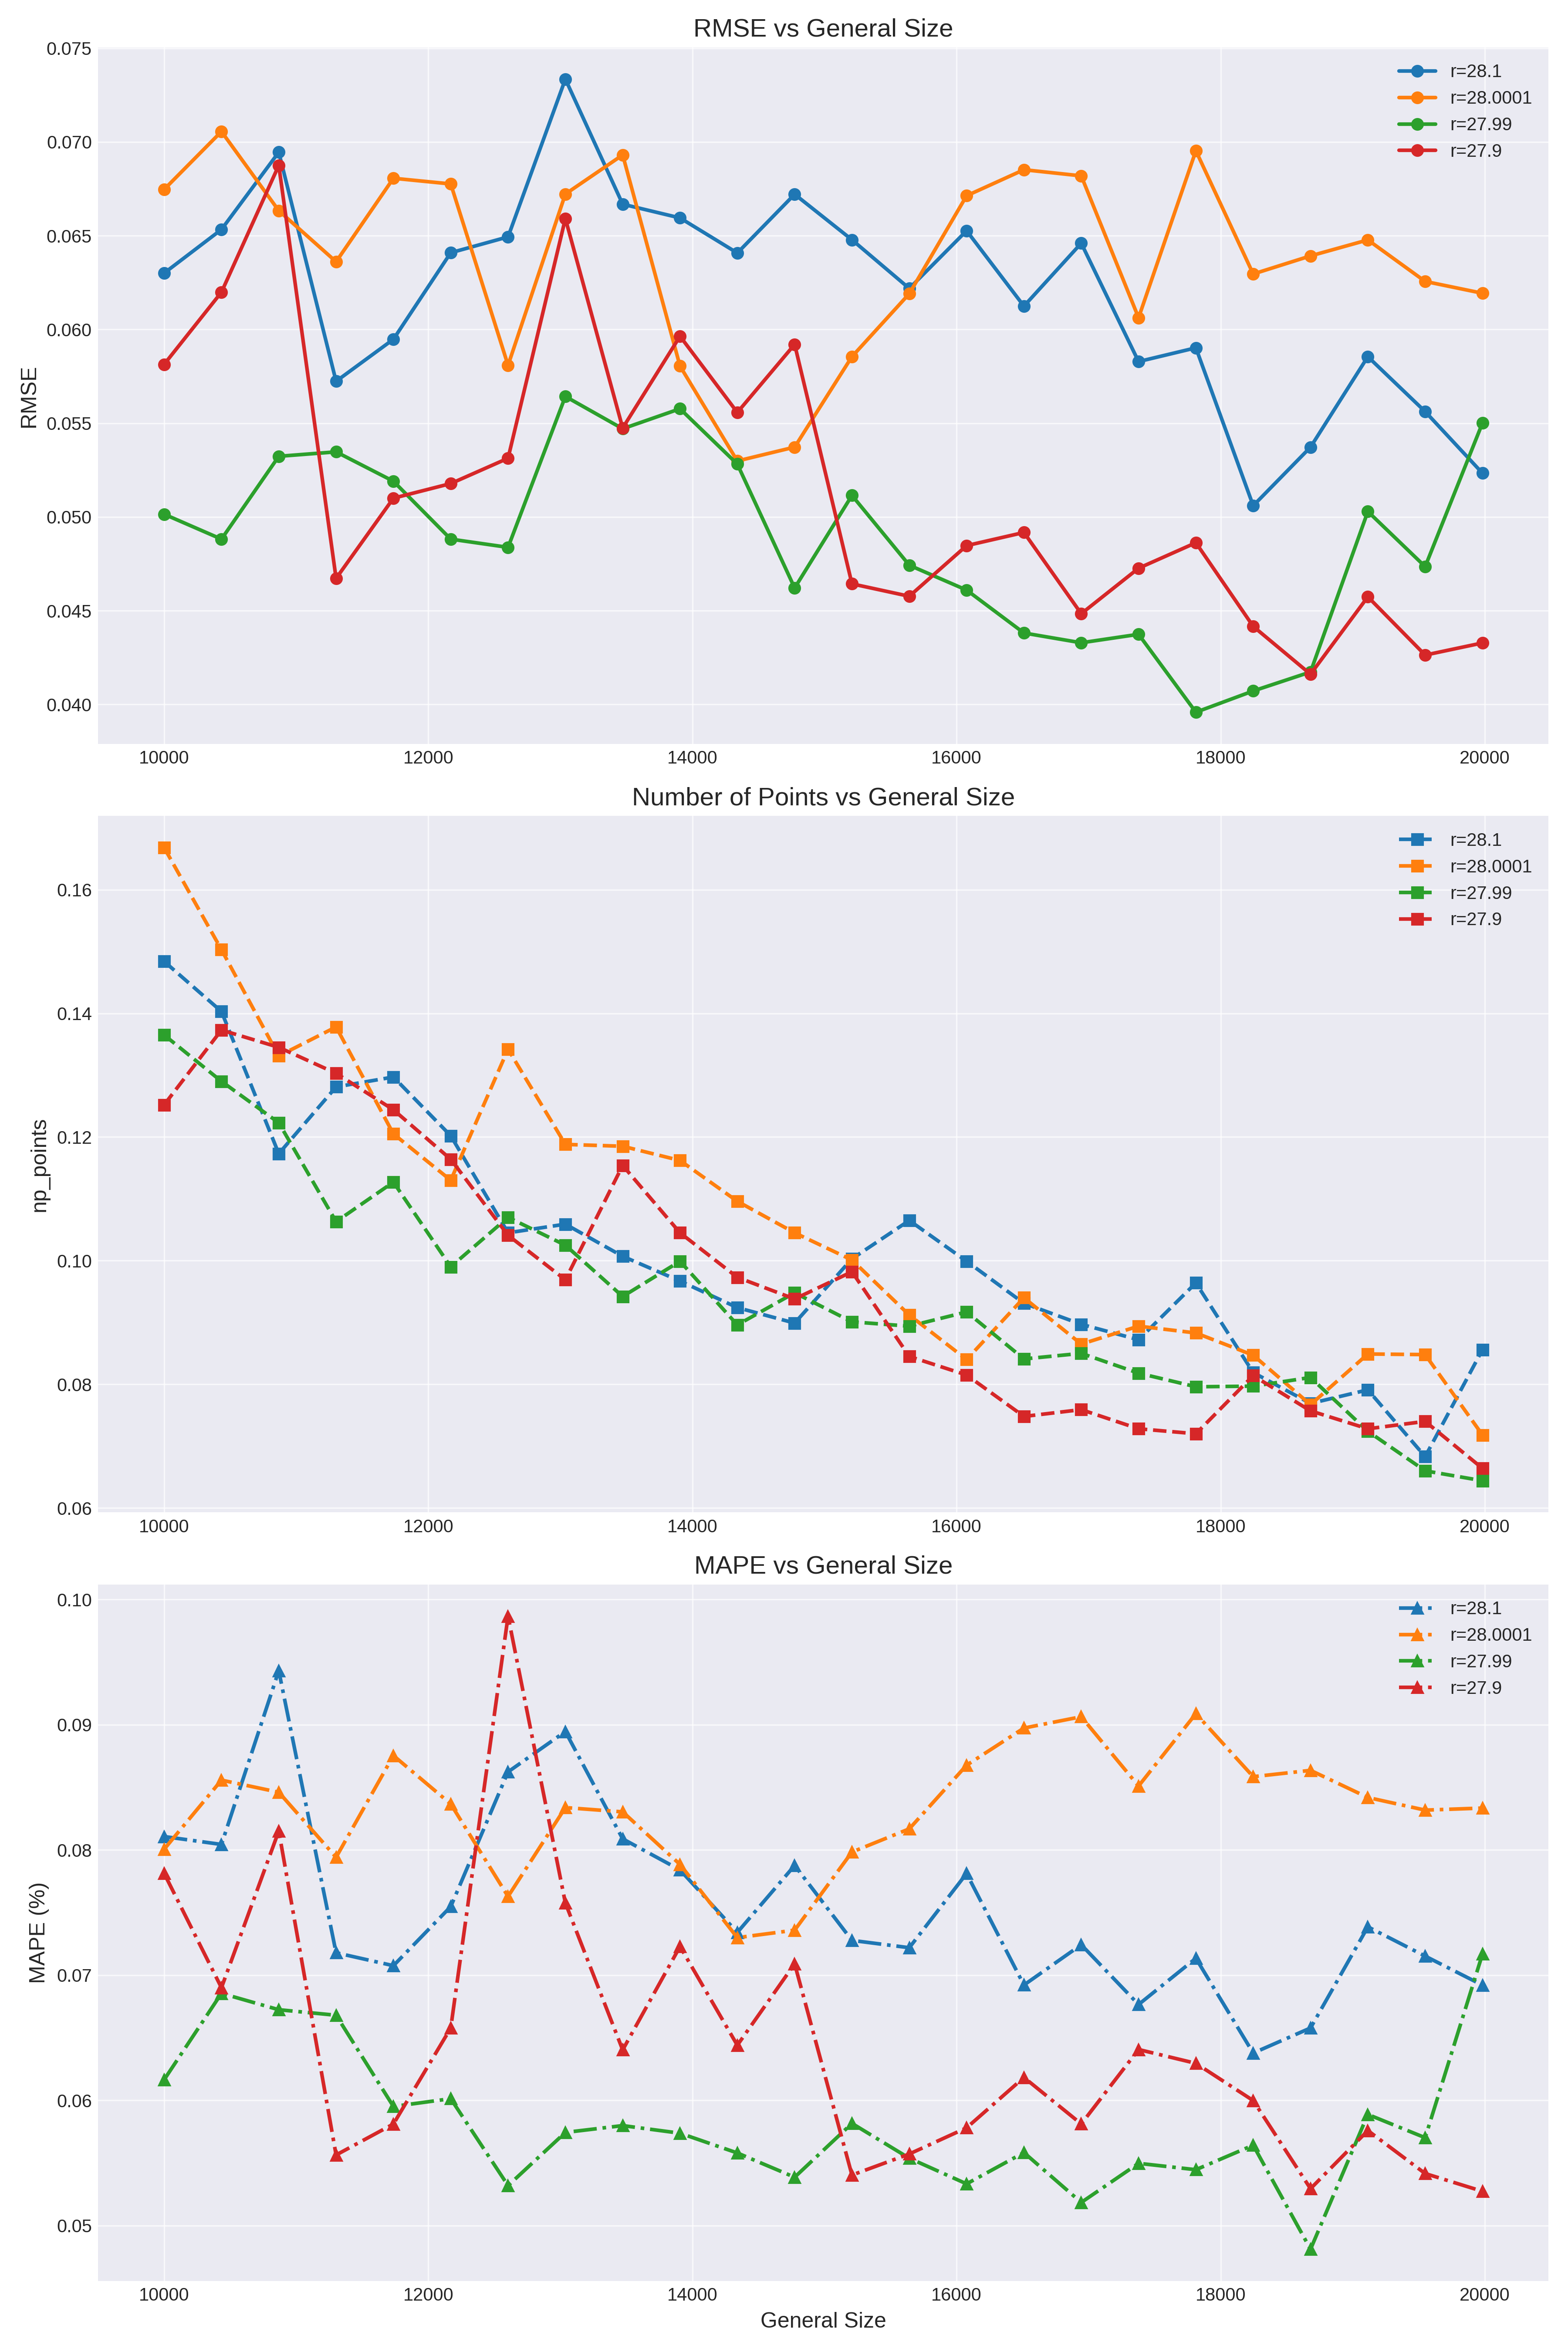
\includegraphics[width=\textwidth]{../Size_experiment/metrics_vs_general_size_best_experiments_2.png}
    \caption{Зависимость метрик от размера выборки для эффективных параметров без использования векторов из основного ряда.}
    \label{fig:main_exp_2}
\end{figure}
Результаты (Рис. \ref{fig:main_exp_2}) показывают, что с увеличением размера в
ыборки из вспомогательных рядов доля непрогнозируемых точек устойчиво снижается,
 однако метрики RMSE и MAPE падают незначительно. Это говорит о том, что модель 
 способна изучить общую динамику аттрактора по данным из систем со схожей динамикой,
  что позволяет ей избегать неопределенности, но для достижения высокой
   точности ей необходимы данные непосредственно из целевой траектории.
    Однако, как и в предыдущем эксперименте, эффективность зависит от
     выбора параметров: метрики качества крайне шумные и высокие по сравнению с выборкой,
     в которой присутствуют z-вектора из основного ряда.
      или NP в шесть раз, и в некоторых случаях метрики ухудшаются в несколько раз.

\subsection{Эксперимент 3: Систематическое исследование параметра r}
\begin{figure}[htbp]
    \centering
    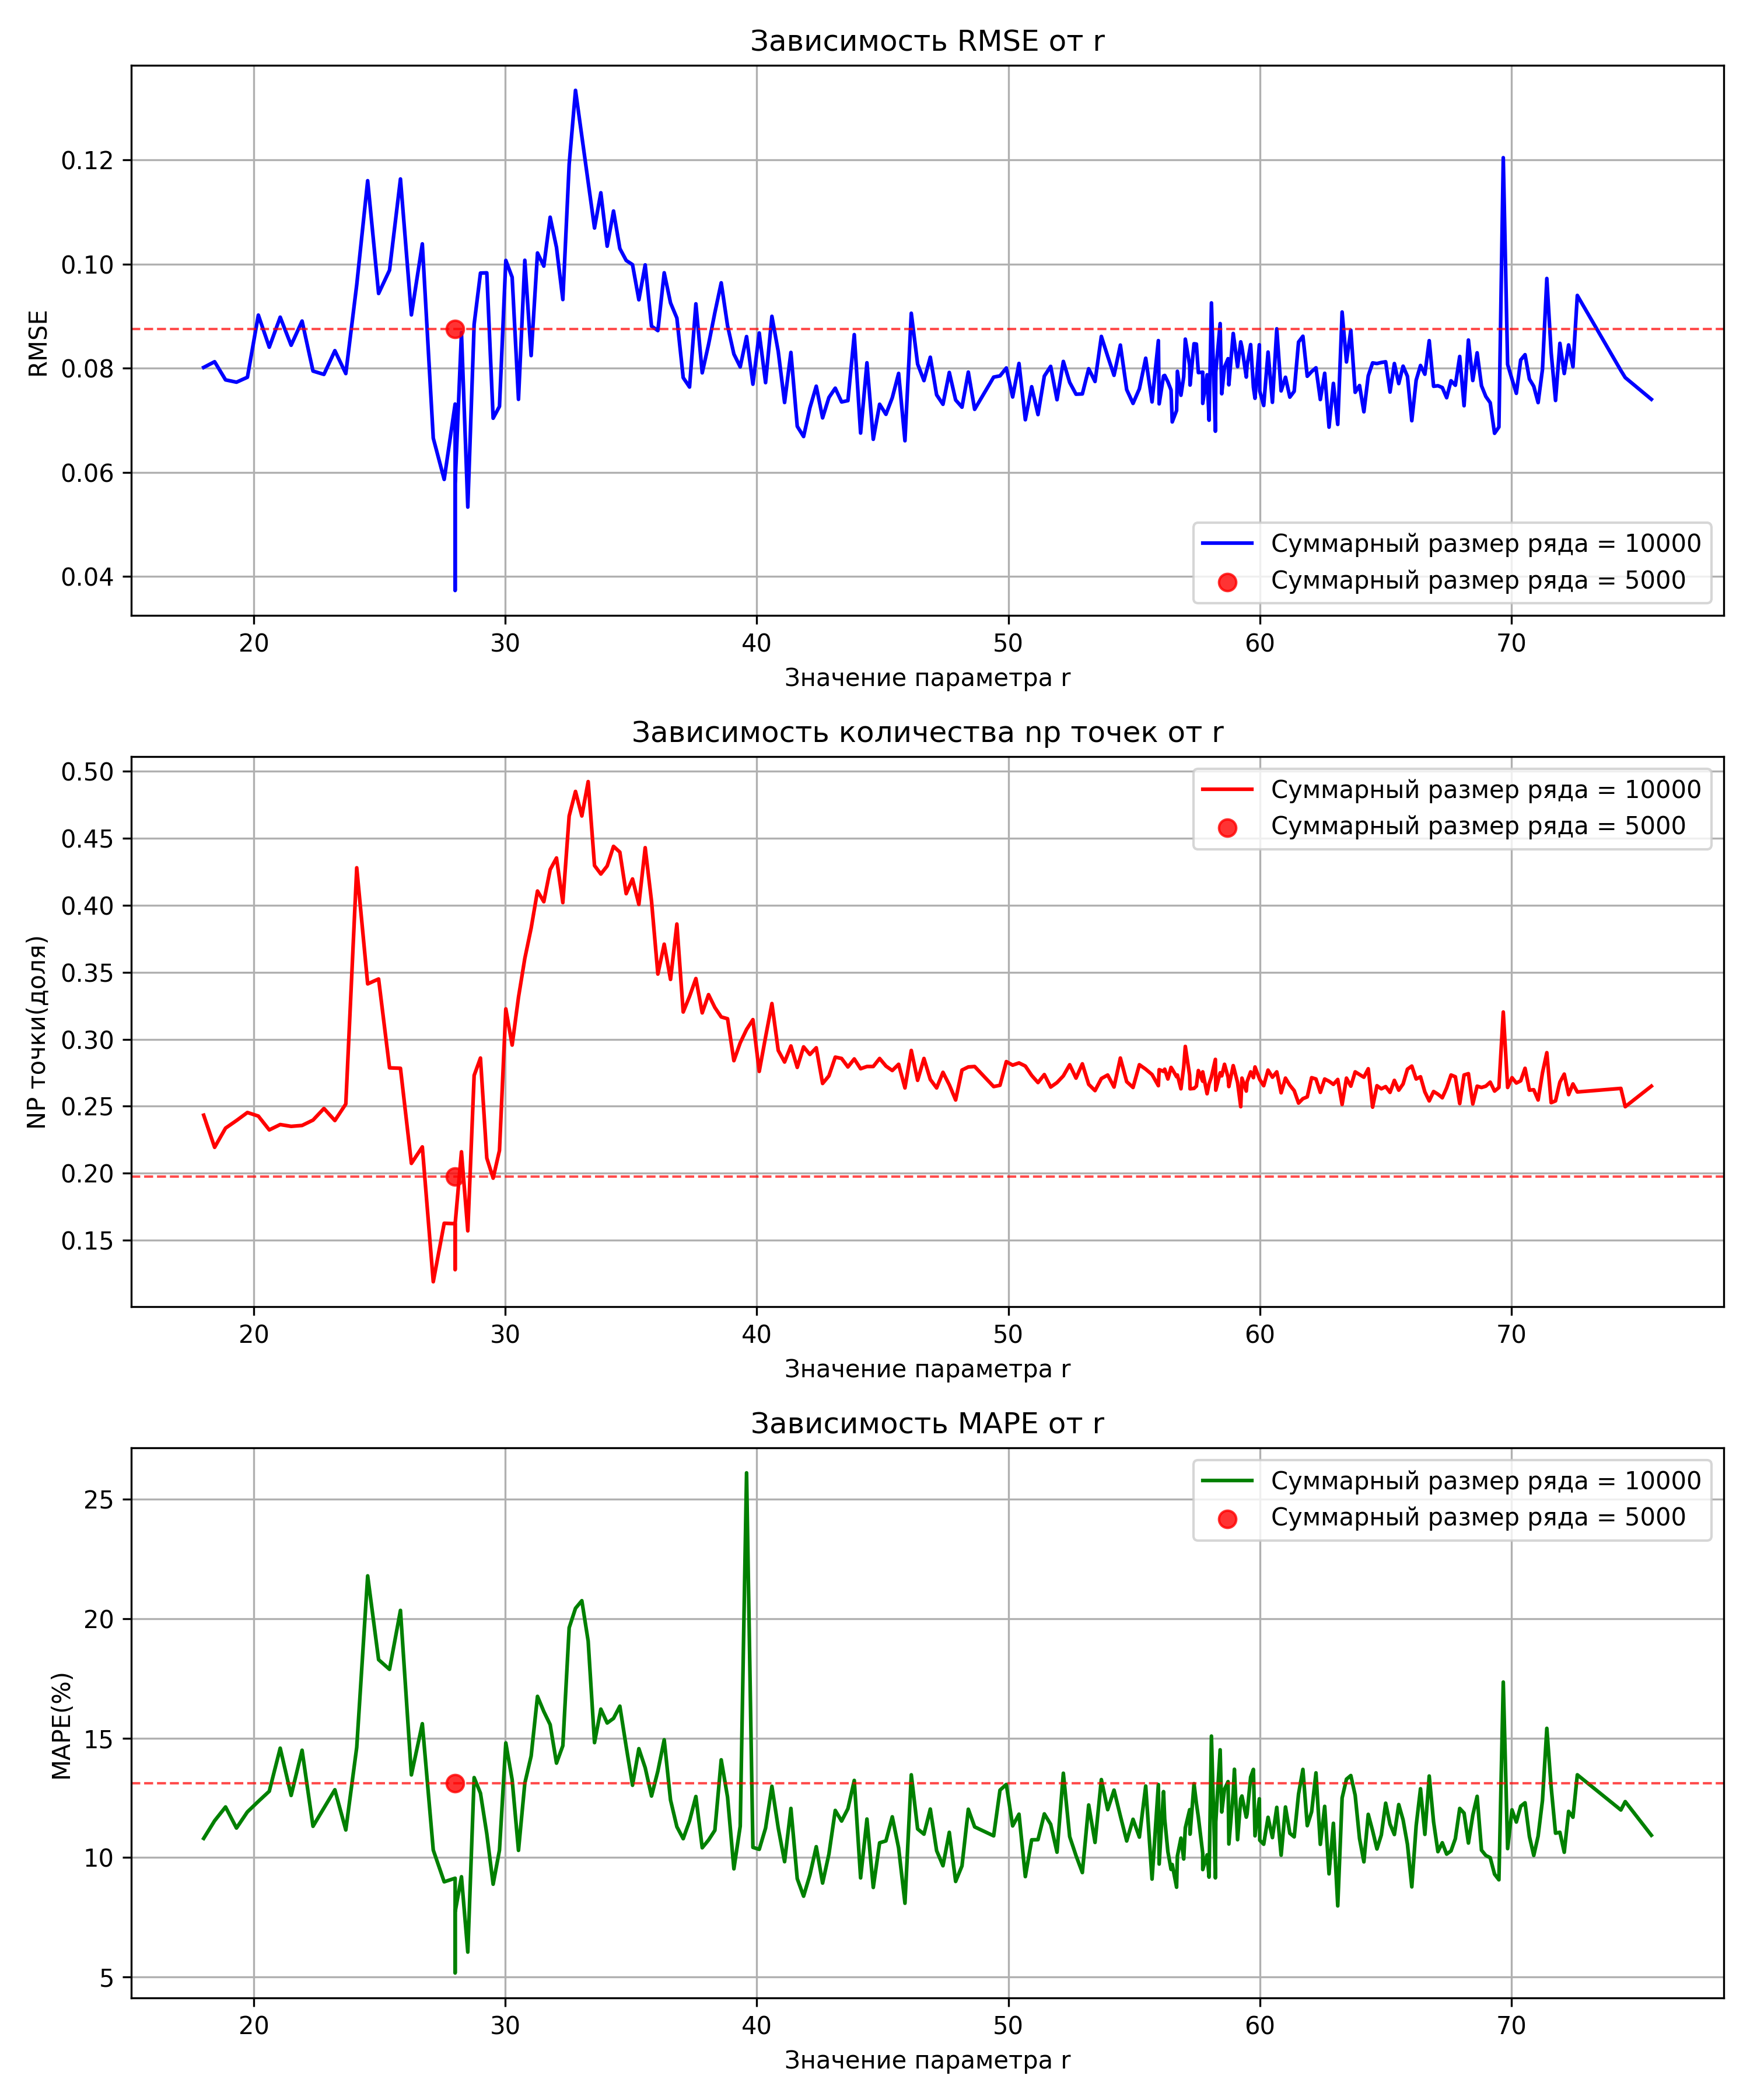
\includegraphics[width=0.8\textwidth]{../deviations/Разные_r.png}
    \caption{Сравнение метрик при добавлении 5000 точек из ряда с различным параметром r к 5000 точкам основного ряда.}
    \label{fig:different_r}
\end{figure}
Результаты (Рис. \ref{fig:different_r}) показывают, что существует узкая окрестность (26,30)
 вокруг `r=28`, в которой добавление вспомогательных рядов приводит к
  улучшению метрик по сравнению с базовой выборкой из 5000 точек. Эта окрестность 
  никак не связана с бифуркационной картиной
  В лучших случаях достигается снижение RMSE и NP в 1.5 раза.
   Однако даже в лучших случаях качество прогноза уступает результатам,
    полученным на выборке из 10000 точек исходного ряда. 
\subsection{Эксперимент 4: Анализ смещения центроидов}
\begin{figure}[htbp]
    \centering
    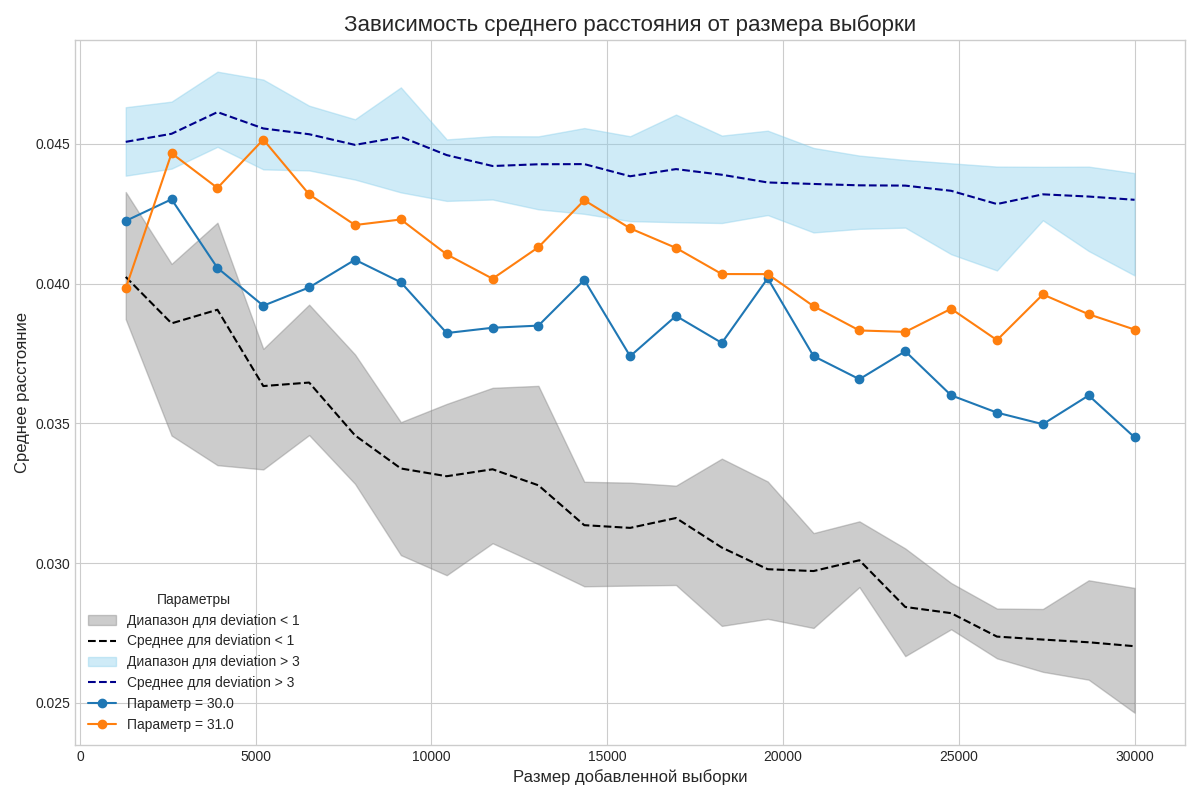
\includegraphics[width=0.8\textwidth]{../centroids_diff/plot_avg_distance.png}
    \caption{Среднее евклидово расстояние между мотивами основного ряда и смешанной выборки.}
    \label{fig:avg_distance}
\end{figure}
Наблюдается (Рис. \ref{fig:avg_distance}), что при добавлении 
значительного объема данных из вспомогательного ряда, среднее
 расстояние между центроидами начинает снижаться логарифмически.
  Это может указывать на то, что добавленные данные стабилизируют
   кластерную структуру, делая центроиды более устойчивыми. 
\section{Заключение}
Проведенное исследование демонстрирует, что метод расширения
 обучающей выборки за счет добавления данных из схожих динамических
  систем является эффективной стратегией для повышения качества прогнозирования
   хаотических временных рядов при ограниченном объеме исходных данных.

Основным преимуществом данного подхода является существенное снижение доли
 непрогнозируемых точек (до 6 раз) и RMSE (до 2 раз), что повышает робастность
  и практическую применимость модели.Также добавление новых рядов может улучшать предсказание даже лучше,
   чем добавление точек исходного ряда(например для r = 27.99).
    Установлено, что такой результат достигается при сохранении точности прогнозирования (RMSE, MAPE) на
    сопоставимом уровне только в том случае, когда вспомогательные данные
     генерируются динамической системой с параметрами, находящимися в малой 
     окрестности параметров целевой системы. При значительном расхождении параметров
      наблюдается существенная деградация точности, что ограничивает применимость метода.
       Кроме того, даже при близких параметрах метод не всегда работает эффективно, как 
       в случае с r=28.01, где метрики остаются на исходном уровне.
    При этом качество добавленного ряда не описывается простыми метриками сравнения двху рядов,вроде DTW
     и корреляции,поскольку не наблюдалось закономерности между качеством прогноза и их значениями
Таким образом, предложенный подход может служить эффективным средством для повышения
 надежности моделей прогнозирования. Направлениями для дальнейших исследований 
 могут стать разработка формальных критериев для определения "схожести" динамических
  систем и применение данного подхода к реальным данным, например, в области
   финансового анализа или медицине.

\newpage
\printbibliography[title={Список использованных источников}]
@book{Aggarwal2013,
  author    = {Aggarwal, C. C. and Reddy, C. K.},
  title     = {Data Clustering: Algorithms and Applications},
  publisher = {CRC Press},
  year      = {2013},
  address   = {Boca Raton, FL, USA}
}

@book{Balashova1991,
  author    = {Balashova, Svetlana D.},
  title     = {Numerical Methods for Solving Differential and Integral Equations. Textbook},
  publisher = {DGU Publishing House},
  year      = {1991}
}

@article{Wang2019,
  author  = {Wang, R. and Peng, C. and Gao, J. and Gao, Z. and Jiang, H.},
  title   = {A dilated convolution network-based LSTM model for multi-step prediction of chaotic time series},
  journal = {Computational and Applied Mathematics},
  year    = {2019},
  volume  = {39},
  number  = {1}
}

@book{Gilmore1984,
  author    = {Gilmore, Robert},
  title     = {Applied Catastrophe Theory, Vol. 2},
  publisher = {Mir Publishers},
  year      = {1984}
}

@inproceedings{Gromov2021,
  author    = {Gromov, Vasilii A.},
  title     = {Chaotic Time Series Prediction: Run for the Horizon},
  booktitle = {CCIS, volume 1288},
  year      = {2021}
}

@article{GromovBaranov2023,
  author  = {Gromov, Vasilii A. and Baranov, Philip S.},
  title   = {Prediction after a Horizon of Predictability: Nonpredictable Points and Partial Multistep Prediction for Chaotic Time Series},
  journal = {Complexity},
  year    = {2023}
}

@misc{Hateley2016,
  author = {Hateley, James},
  title  = {The Lorenz system},
  year   = {2016},
  url    = {http://web.math.ucsb.edu/jhate-ley/paper/lorenz.pdf}
}

@article{KaplanYorke1979,
  author  = {Kaplan, James L. and Yorke, James A.},
  title   = {Preturbulence: A Regime Observed in a Fluid Flow Model of Lorenz},
  journal = {Commun. Math. Phys.},
  year    = {1979},
  volume  = {67},
  pages   = {93-108}
}

@book{MalinetskiyPotapov2002,
  author    = {Malinetskiy, G. G. and Potapov, A. B.},
  title     = {Modern Problems of Non-linear Dynamics},
  publisher = {Editorial URSS},
  year      = {2002},
  address   = {Moscow, Russia}
}

@article{PerezChacon2018,
  author  = {Perez-Chacon, Ruben and Luna Romera, Jose M. and Troncoso, Alicia and Martinez-Alvarez, Francisco and Riquelme, Jose C.},
  title   = {Big Data Analytics for Discovering Electricity Consumption Patterns in Smart Cities},
  journal = {Energies},
  year    = {2018},
  volume  = {11},
  number  = {3},
  pages   = {683}
}

@incollection{Takens1981,
  author    = {Takens, F.},
  title     = {Detecting strange attractors in turbulence},
  booktitle = {Dynamical Systems and Turbulence},
  series    = {Lecture Notes in Mathematics},
  volume    = {898},
  publisher = {Springer-Verlag},
  year      = {1981},
  pages     = {366-381}
}
\end{document}